\documentclass{article}
\usepackage{tikz}
\begin{document}
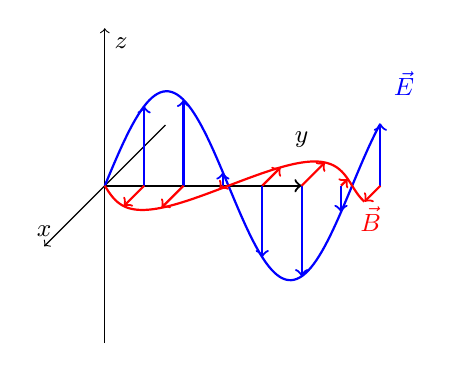
\begin{tikzpicture}[scale=1, every node/.style={font=\small}]
    \draw[->] (0,-2,0) -- (0,2,0) node[anchor=north west] {$z$};
    \draw[->] (0,0,-2) -- (0,0,2) node[anchor=south] {$x$};
    \draw[->, thick] (0,0,0) -- (2.5,0,0) node[above=10pt] {$y$};
    \draw[thick, blue, domain=0:3.5, samples=100] 
        plot (\x, {1.2*sin(2*\x r)}, 0);
    \foreach \x in {0.5,1.0,...,3.5} {
        \draw[->, thick, blue] (\x,0,0) -- (\x, {1.2*sin(2*\x r)}, 0);
    }
    \node[blue] at (3.8,1.3,0) {$\vec{E}$};
    \draw[thick, red, domain=0:3.5, samples=100] 
        plot (\x, 0, {0.8*sin(2*\x r)});
    \foreach \x in {0.5,1.0,...,3.5} {
        \draw[->, thick, red] (\x,0,0) -- (\x, 0, {0.8*sin(2*\x r)});
    }
    \node[red] at (3.8,0,1.1) {$\vec{B}$};
\end{tikzpicture}

\end{document}